\section{System Block}

\begin{figure}[h]
  % \def\svgwidth{\columnwidth}
  % \includesvg{mainmatter/3-Methodology/images/block.svg}
  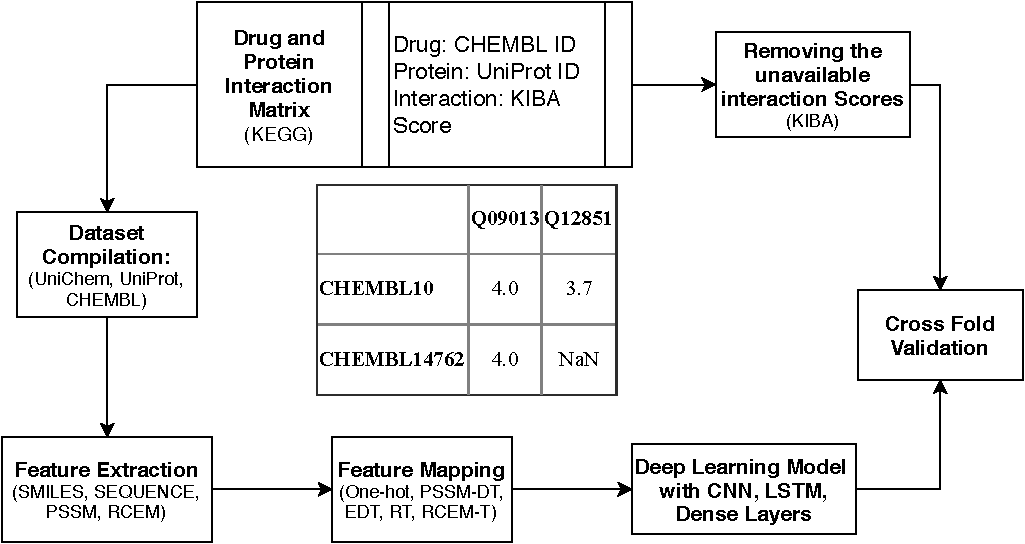
\includegraphics[width=1\linewidth]{mainmatter/3-Methodology/images/block.pdf}
  \caption{Schematic Block Diagram for Protein-Drug Prediction}
  \label{fig:system}
\end{figure}

The Figure ~\ref{fig:system} shows the various components used to form the prediction system. The idea is basic in that protein interaction depends on the structural and chemical properties. The primary canonical structure of protein-drug set are fed into interaction block. The interaction parameter is filtered accordingly to the filter type. Similarly, the drug feature set are created to be trained with the machine learning algorithm. Finally, after training the training dataset, we cross validate the model with test dataset.


\section{Dataset Description}

\iffalse
\subsection{\acrfull{kegg}}
\acrfull{kegg} is a community-driven database which contains large-scale molecular datasets generated by genome sequencing and high-throughput experimental techniuqe.\cite{Kanehisa2000, ozturk2018deepdta} We use \acrshort{kegg} DRUG dataset for finding the interaction set between DRUG and PROTEIN. The interaction score is :
\fi

\subsection{\acrfull{kiba}}
The \acrfull{kiba} Scores are collected from the publicly made available dataset \cite[\textit{Tang. et al.}]{Tang2013}. The scores are actually based on thermodynamic constants K\textsubscript{i} and K\textsubscript{d} and, remaining enzyme activity(Activity \% --  IC\textsubscript{50}) .

% \begin{flushright}
\begin{equation}
  KIBA = \begin{cases}
    K_i . {adj} & \quad {if} \; {IC_{50}\: and\, K_i \,are\, present} \\
    K_b.{adj} & \quad {if}  {IC_{50} \, and \, K_d \, are \, present} \\
    \frac{K_i . {adj} \; K_b.{adj}}{2} & \quad {if\, IC_{50}\,,K_i\, and \,K_d\, are\, present}
  \end{cases}
   \label{eq:kiba}
\end{equation}
where,
\begin{equation}
K_i.{adj} = \frac{IC_{50}}{1 + L_i(IC_{50}/K_i)}
\label{eq:ki_adj}
\end{equation}

\begin{equation}
K_d.{adj} = \frac{IC_{50}}{1 + L_d(IC_{50}/K_d)}
\end{equation}
where L\textsubscript{d} and L\textsubscript{i} are parameters defining weights of IC\textsubscript{50} in model adjustments for K\textsubscript{i} and K\textsubscript{b} 
% \end{flushright}

For a kinase inhibitor drug−target interaction, we consider the medians of three major bioactivity types IC\textsubscript{50}, K\textsubscript{i}, K\textsubscript{d} where
IC\textsubscript{50} \cite{Tang2013} is the concentration at which the inhibitor causes a 50\% inhibition of enzymatic activity and K\textsubscript{i} is defined by \begin{equation}
    Ki = \frac{IC_{50}} {1 + [S]  K_m}
    \label{eq:ki}
\end{equation} 
where,  [{S}] is the experimental substrate concentration and K\textsubscript{m} is the concentration of the substrate.

\iffalse
\begin{equation}
    \tau= \frac{(a−b)}{n(n − 1)/2}   
    \label{eq:tau}
  \end{equation}
  { Here {a} and {b} represent the number of concordant pairs and discordant pairs respectively. }
\fi


All the bioactivity types are available from CHEMBL\cite{Gaulton2017}. Based on interaction data available, we remove the unknown values and get a total of 180244 interaction KIBA score values in the range of -3.09 to 17.8. With the standard deviation of 1.22, it represents a total of \arabic{no_proteins} proteins and \arabic{no_drugs} drugs.

\subsection{Position Specific Score Matrix}

\acrfull{pssm} is a very useful protein feature. The protein feature represented by PSSM depends on the sequence of all the proteins in consideration. The HUMAN genome protein (a database of more than 100,000) is downloaded from UniProt Library. The PSSM matrix is constructed for each of the kinase proteins based on this HUMAN Genome Protein Database. With this, the PSSM matrix is characterized according to human proteins to anticipate the prediction of new identified kinase proteins.

\begin{table}
  \centering
  {\caption{PSSM Analysis Design}
  \label{table:PSSM_Analysis} }
    \subfloat[][Protein FASTA Sequence]{
      \label{table:PSSM_Analysis:fasta} 
      \begin{tabular}{|l|l|} \toprule
      \hline
      1 & GAGGTAAAC \\ \hline
      2 & TCCGTAAGT \\ \hline
      3 & CAGGTTGGA \\ \hline
      4 & ACAGTCAGT \\ \hline
      5 & TAGGTCATT \\ \hline
      6 & TAGGTACTG \\ \hline
      7 & ATGGTAACT \\ \hline
      8 & CAGGTATAC \\ \hline
      9 & TGTGTGAGT \\ \hline
      10 & AAGGTAAGT \\ \hline
      
      \end{tabular}
    }
    \subfloat[][Frequency Table]{
      \label{table:PSSM_Analysis:frequency}
      \begin{tabular}{|l|l|l|l|l|l|l|l|l|l|} \toprule
        \hline
        
         & 1 & 2 & 3 & 4 & 5 & 6 & 7 & 8 & 9 \\ \hline
        A & 3 & 6 & 1 & 0 & 0 & 6 & 7 & 2 & 1 \\ \hline
        C & 2 & 2 & 1 & 0 & 0 & 2 & 1 & 1 & 2 \\ \hline
        G & 1 & 1 & 7 & 10 & 0 & 1 & 1 & 5 & 1 \\ \hline
        T & 4 & 1 & 1 & 0 & 10 & 1 & 1 & 2 & 6 \\ \hline
        
        \end{tabular}

    } 
  
  
  \subfloat[][Log-Likelihood Matrix]{
    % \rule{4cm}{0cm}
    \begin{tabular}{|l|l|l|l|l|l|l|l|l|l|} \toprule
      \hline 
  
          & 1 & 2 & 3 & 4 & 5 & 6 & 7 & 8 & 9 \\ \hline
      A & 0.3 & 0.6 & 0.1 & 0.00 & 0.00 & 0.6 & 0.7 & 0.2 & 0.1 \\ \hline
      C & 0.2 & 0.2 & 0.1 & 0.00 & 0.00 & 0.2 & 0.1 & 0.1 & 0.2 \\ \hline
      G & 0.1 & 0.1 & 0.7 & 1.00 & 0.00 & 0.1 & 0.1 & 0.5 & 0.1 \\ \hline
      T & 0.4 & 0.1 & 0.1 & 0.00 & 1.00 & 0.1 & 0.1 & 0.2 & 0.6 \\ \hline
      
      \end{tabular}  
      \label{table:log_likelihood_pssm}
    }
    
  
  \subfloat[][Sliding Window Score Calculation]{
    \centering
    \begin{tabular}{|l|l|l|l|l|l|l|l|l|l|}
    \hline 
    
        & 1 & 2 & 3 & 4 & 5 & 6 & 7 & 8 & 9 \\ \hline
    A & 0.3 &  &  &  &  &  & 0.7 &  &  \\ \hline
    C &  &  & 0.1 & 0.00 & 0.00 & 0.20 &  &  & 0.2 \\ \hline
    G &  & 0.1 &  &  &  &  &  & 0.5 &  \\ \hline
    T &  &  &  &  &  &  &  &  &  \\ \hline
    
    \end{tabular}  
    \label{table:motif_movement}
    }

    
    \subfloat[][Score of sliding window motifs]{
    \label{wrapTable:pssm-score}
    \begin{tabular}{|l|l|l|l|l|l|l|l|l|l|}
      \hline
      0 & 1 & 2 & 3 & 4 & 5 & 6 & 7 & 8 & 9 \\ \hline
      1.099 & 1 & 2.2 & 2.1 & 2.1 & 1.300 & 1.3 & 1.4 & 2 & 2.9 \\ \hline
      \end{tabular}
    }
\end{table}

Table \ref{table:PSSM_Analysis} shows a conventional process of calculating PSSM score values. The sequence following shows the process of calculating the scores once the PSSM distribution of the whole family is calculated. Table \ref{table:motif_movement} shows the score distribution of lowercase amino acid sequence (starting after 4th position) determined by the size of the sliding window.

\seqsplit{ACTC\textbf{agccccagc}GGAGGTGAAGGACGTCCTTCCCCAGGAGCCGGTGAGAAGCGCAGTCGGGGGCACGGGGATGAGCTCAGGGGCCTCTAGAAAGATGTAGCTGGGACCTCGGGAAGCCCTGGCCTCCAGGTAGTCTCAGGAGAGCTACTCAGGGTCGGGCTTGGGGAGAGGAGGAGCGGGGGTGAGGCCAGCAGCA} 

% % \begin{wraptable}{br}{5.5cm}
% \begin{table}[H]
%     \centering
    
% \end{table}
% % \end{wraptable}

.3, .1, .1, 0, 0, .2, .7, .5, .2  == Sum(2.1) - posix(4) -- See table \ref{wrapTable:pssm-score}

\begin{figure}[htbp]
    \centering 
          %  \subfloat[]{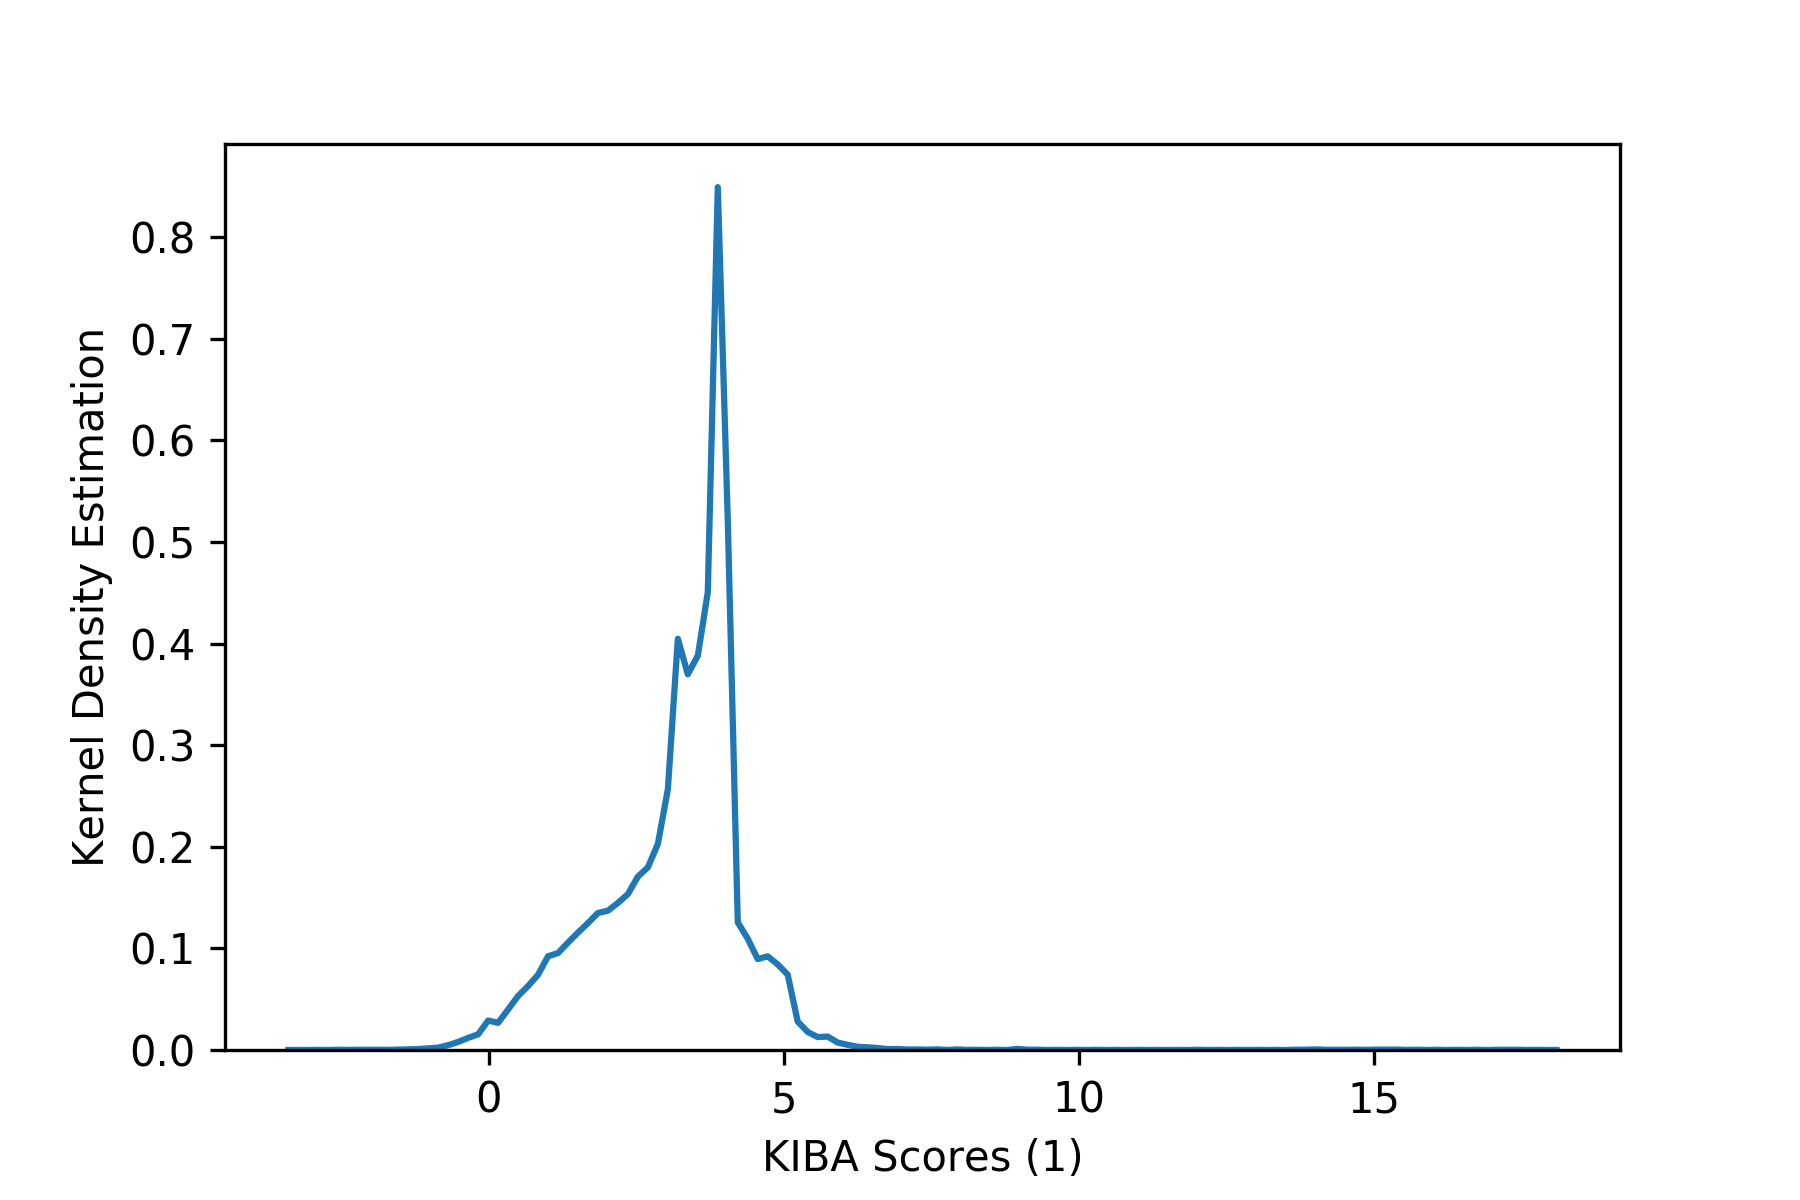
\includegraphics[width=.3\textwidth]{dataset/images/KIBA_scores.png}}
          
           \subfloat[][Drug-Protein Interaction]{
             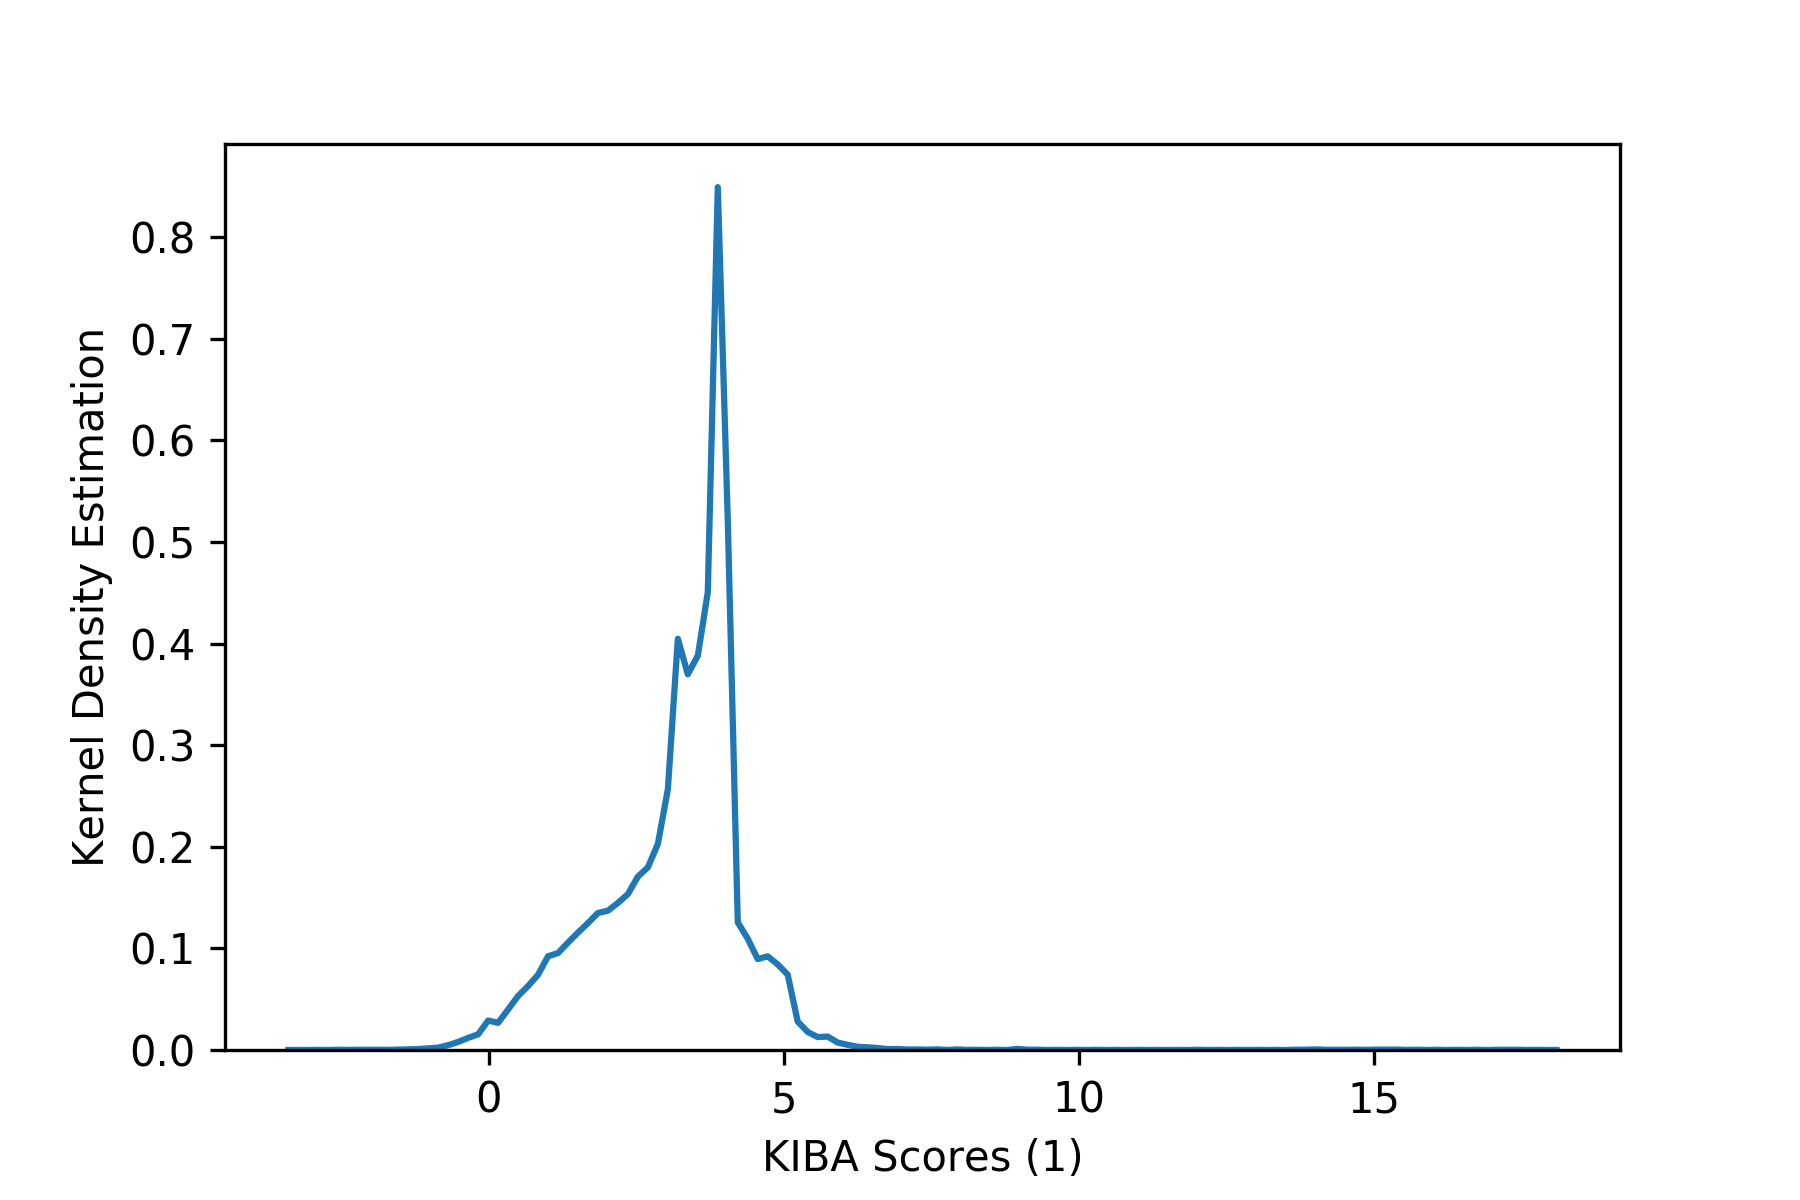
\includegraphics[width=.5\textwidth]{dataset/images/KIBA_scores.png}
             \label{fig:kiba_scores}
             }

           \subfloat[][Drugs SMILES Sequence]{
            \label{fig:drug_dist}  
            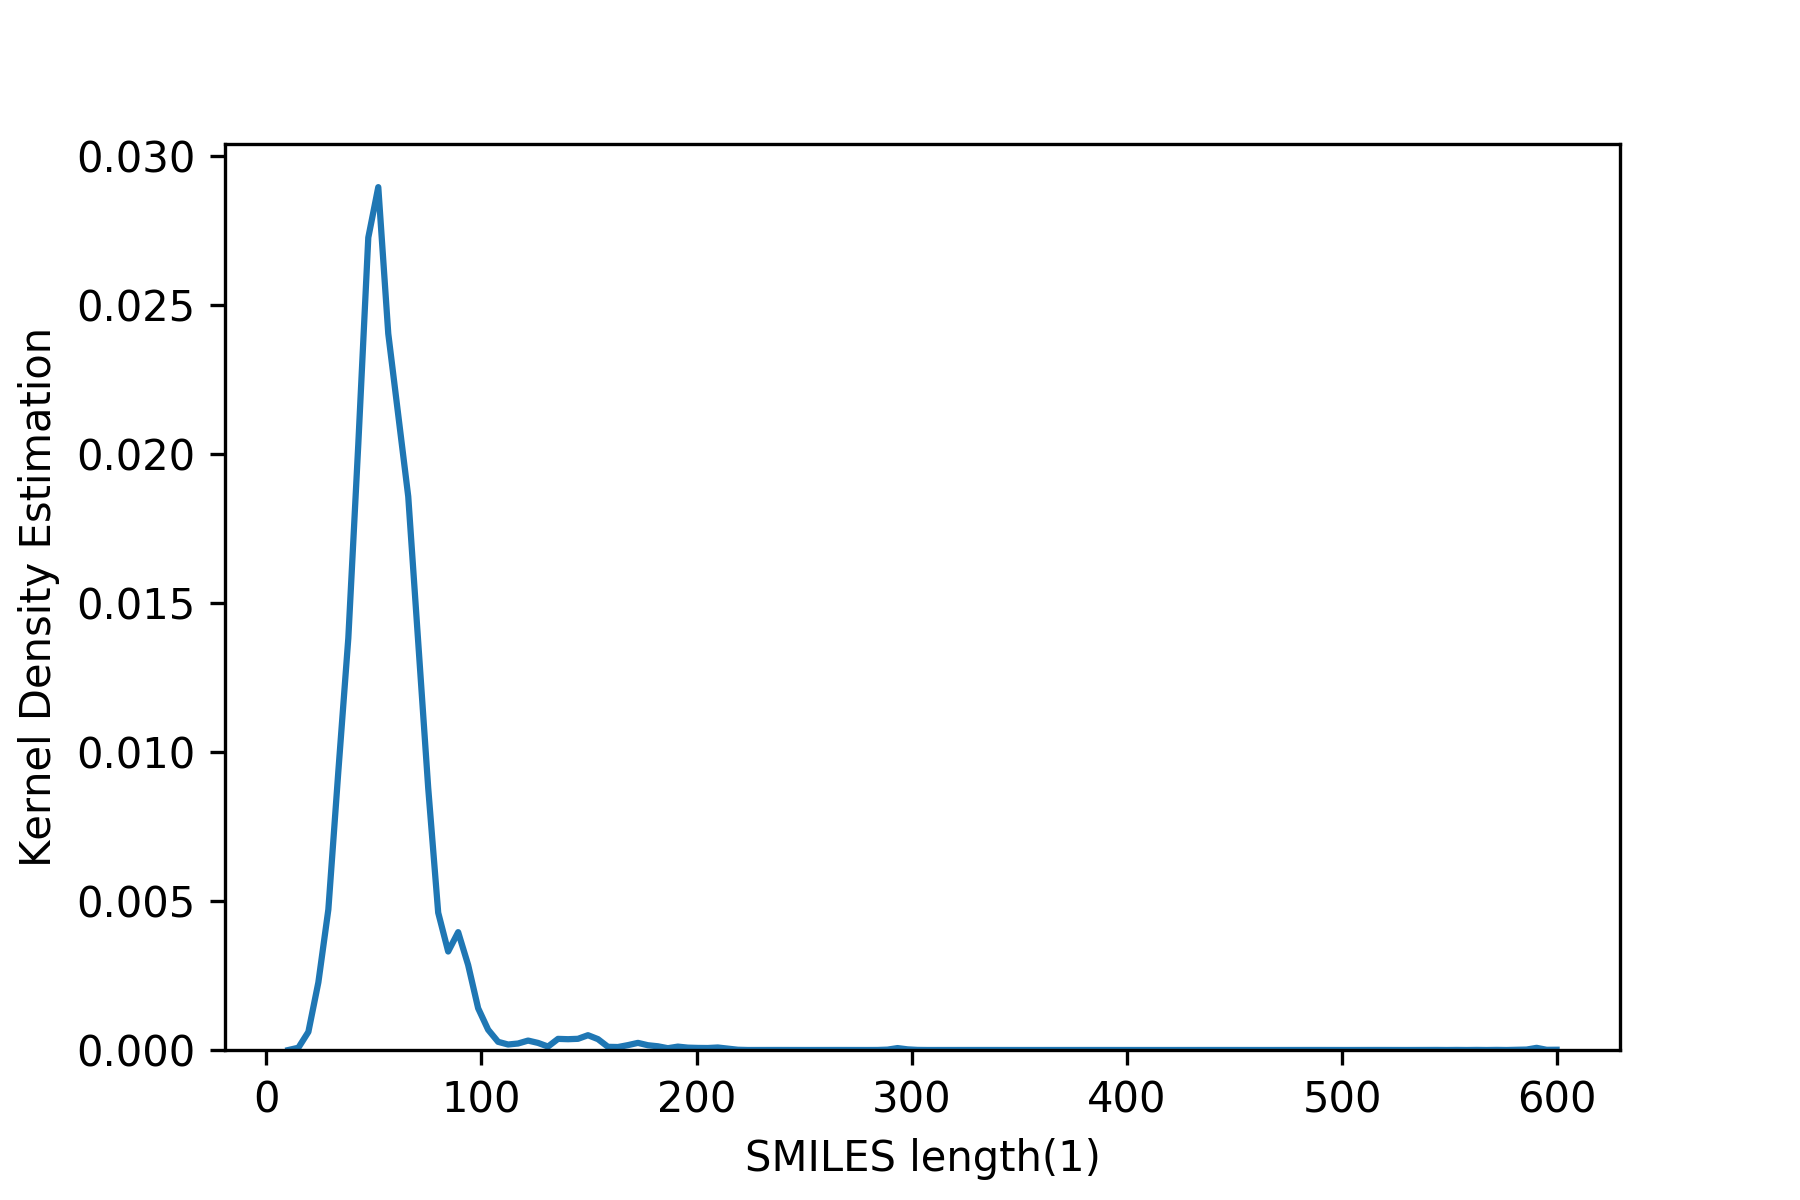
\includegraphics[width=.5\textwidth]{dataset/images/SMILES_distribution.png}
            }

           \subfloat[][Protein FASTA Sequence]{
             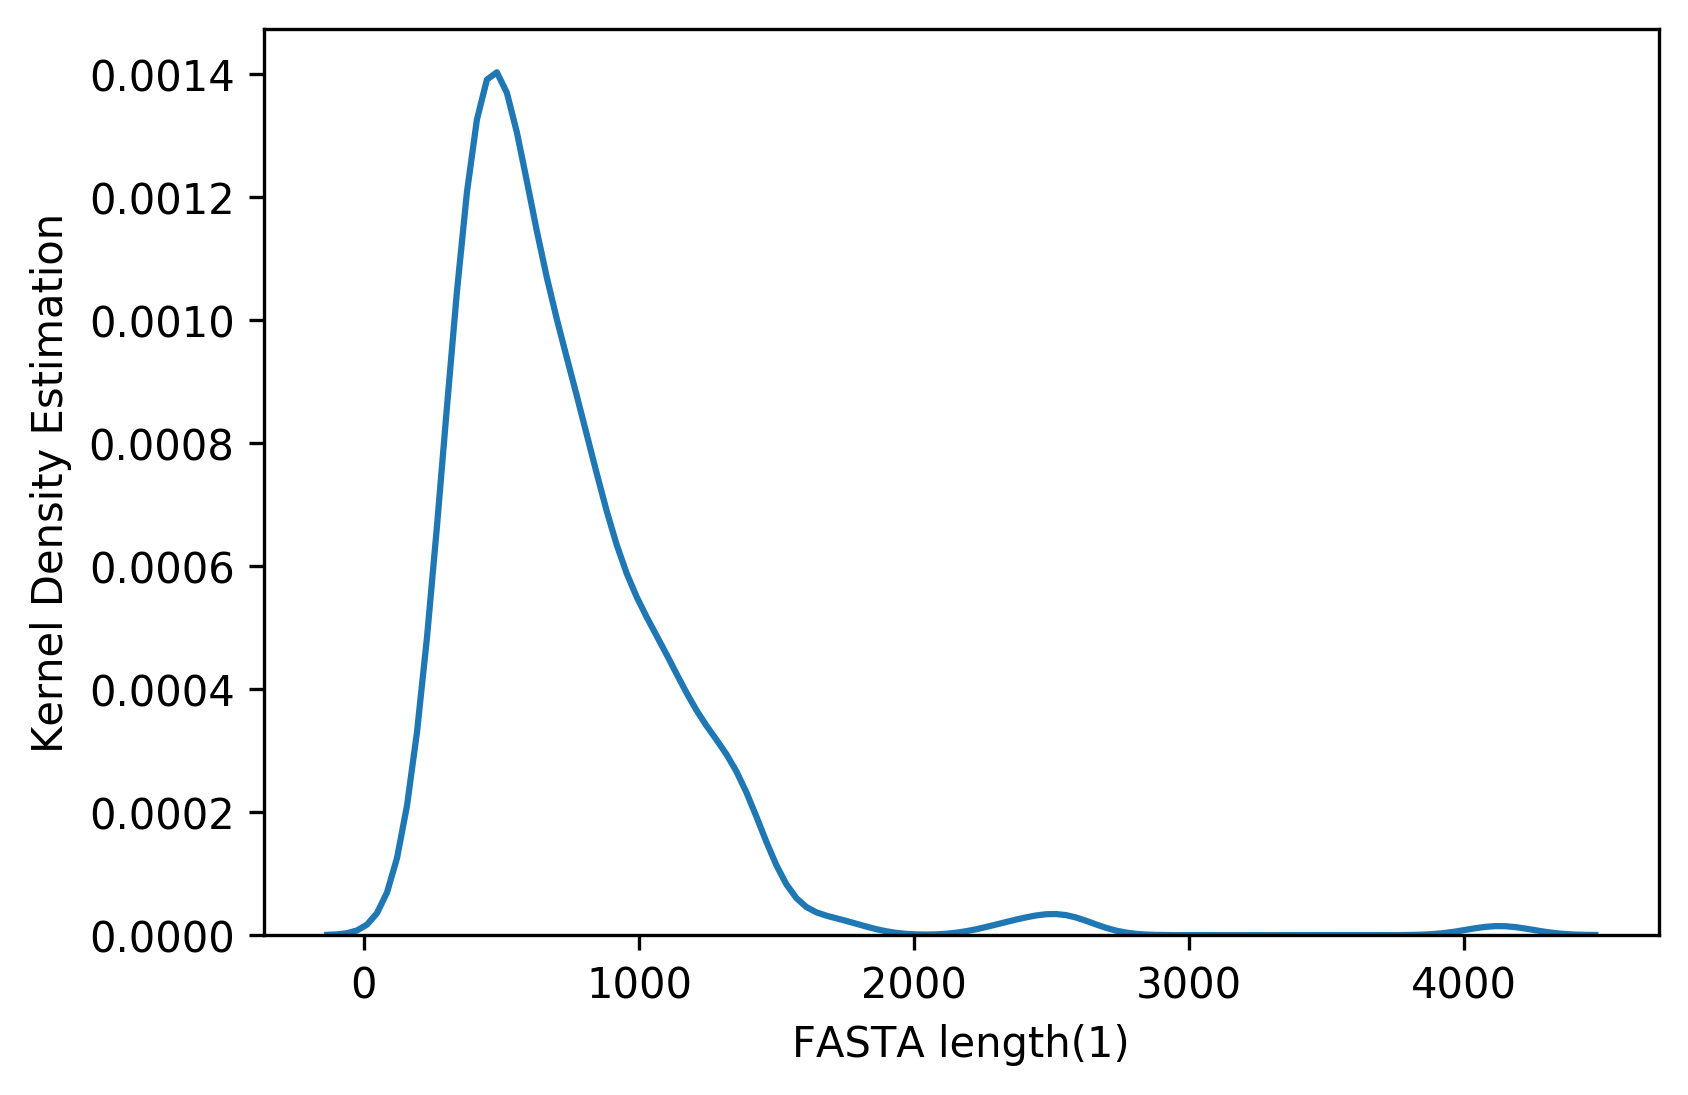
\includegraphics[width=.5\textwidth]{dataset/images/FASTA_distribution.png}
             \label{fig:prot_dist}
            }

           \caption[KDE Distribution]{Kernel Density Estimation Distribution of KIBA-interaction scores of Drug Sequences and Protein Sequences. \ref{sub@fig:kiba_scores} Distribution of KIBA Scores in Protein-Drug Interaction Pair, \ref{sub@fig:drug_dist} Distribution of length in Labeled Encodings of Drug Sequence, \ref{sub@fig:prot_dist} Distribution of length in Labelled Encodings Protein Sequence }
           \label{fig:kiba_drug_protein}
\end{figure}
  
\iffalse
  \subsection{UniProt and CHEMBL}
  
  \subsubsection{UniProt} 
  The sequence related information of protein is referenced using UniProt Identifier and protein sequence (FASTA) is called using the api from UniProt. \cite{UniProtConsortium2018}
  
  
  \subsubsection{CHEMBL}
  The molecular fingerprints related to drugs are referenced usning CHEMBL Identifier and the drug sequence is called from CHEMBL database. \cite{Gaulton2017}
  \fi
  \subsection{PSI-BLAST}
  PSI-Blast tools relates with multiple sequence alignments from a family of protein sequences\cite{Schaffer2001}. This helps to create a \acrshort{pssm} - Equation (\ref{eq:pssm}) - matrix referred to as secondary protein structure. For this study, the PSSM profile of every protein sequence is obtained by executing iteration of PSI-BLAST against \cite[KEGG]{Schaffer2001} protein. PSSM profile is a matrix of L*20 dimensions whereby 20 is the standard type of amino acids and L being the length of the protein. The larger positive scores represent conserved positions, which in turn implies critical functional residues that are required to perform various intermolecular interactions.\cite[PSSM]{Schaffer2001}
  
  \begin{equation}
    PSSM = \begin{bmatrix}
      P_{1,1} & P_{1,2} & \dots & P_{1,20} \\
      P_{2,1} & P_{2,2} & \dots & P_{2,20} \\
      \vdots  & \vdots  & \ddots & \vdots \\
      P_{L,1} & P_{L,2} & \dots & P_{L,20} \\
    \end{bmatrix}
    \label{eq:pssm}
  \end{equation}
  
  \subsubsection{PSSM-DT}
  Two forms of \acrshort{pssm} distance transformation techniques are used to transform the \acrshort{pssm} information into fixed dimensional vectors \cite{Xu2015}. The PSSM-DT (PSSM-Distance Transformation) can transform the \acrshort{pssm} information into uniform numeric representation by approximately measuring the occurrence probabilities of any pairs of amino acid. It results in two types of feature matrices: PSSM-SDT and PSSM-DDT defined by:
  
  \begin{equation}[H]
    PSSM-SDT(i,lg) = \sum_{i=1}^{L-lg} S_{i,j} \times \frac{ S_{i,j+lg} }{L-lg} 
    \label{eq:pssmsdt}
  \end{equation}
  \textit{\center lg =  distance of separation between same amino acid sequence}
  
  \begin{equation}[H]
    PSSM-DDT(i_1,i_2, lg) = \sum_{j=1}^{L-lg} S_{i_1,j} \times \frac{ S_{i_2,j+lg} }{ L-lg} 
    \label{eq:pssmddt}
  \end{equation}
  \textit{\centering i\textsubscript{1} and i\textsubscript{2} refer to tow different types of amino acids}
  
  Thus we have [380 ~\eqref{eq:pssmddt}+20 ~\eqref{eq:pssmsdt} = 400] x lg matrix which will be used as protein-specific vector in this work.
  
  \subsubsection{Evolutionary Distance Transformation Matrix}
  The mutational information of protein can be more informative than the sequence information itself\cite{Zhang2014}. Evolutionary difference formula (EDF) is used to represent mutation difference between adjacent residues. Secondly, the PSSM is converted into 20 x 20 matrix (ED-PSSM). These extracts are the non co-occurrence probability for two amino acids separated by a certain distance \textit{d} in the protein from the PSSM profile. For example, d=1 implies that the two amino acids are consecutive; d=2 implies that there is one amino acid between the two. Next, the EDT feature vector computed from ED-PSSM can be represented as (~\ref{eq:Pmat}): 
  \begin{equation}
    \label{eq:Pmat}
    P = [ \partial_1 ,\partial_2, \dots, \partial_\Omega]
  \end{equation}
  where $\Omega$ is an integer that represents the dimension of the vector whose value is 400.. The non-co-occurrence probability of two amino acids separated by distance \textit{d} can be computed as:
  \begin{equation}
    f(A_x,A_y) = \sum_{d=1}^{D} \frac{1}{L-d} \sum_{i=1}^{L-d} (P_{i,x} - P_{i+d,y})^2
    \label{eq:edt}
  \end{equation}
  where $P_{i,x}$ and $P_{i+d,y}$ are the elements in the PSSM profile; $A_x$ and $A_y$ represent any of the the 20 different amino acids in the protein sequence. Finally we spread the $f(A_x,A_y)$ in equation ~\ref{eq:Pmat} as:
  $ \partial_1 = f(A_1,A_2) $, 
  $ \partial_{400} = f(A_{20}, A_{20}) $
  
  
  \subsection{Residue feature} 
  The Statistical Residue Vector Space \acrshort{srv} \cite{Wong2018} plays an important role in Residue Residue Interaction and creates a basis for structural stability of the protein sequence itself. It is related to the tertiary structure of the protein sequence. Nonetheless, another function is to create a correlated sequence of information whereby two proteins are distantly related by sequence. Simultaneously, it is highly related to the functional characteristic of protein.  With this, table ~\ref{table:r2r} as attached in Appendix depicts a 20 x 20 matrix whose rows and columns represent 20 standard amino acids.
  
  \subsubsection{Residue Probing Transformation(RPT) feature}
  RPT as proposed by Jeong et al.\cite{Jeong2011}, and implemented by Pujan et al.\cite{Mishra2019}, emphasize domains with similar conservation rates by grouping domain families based on their conservation score in the PSSM profile.
  \begin{equation}
    RPT = \begin{bmatrix}
      S_{1,1} & S_{1,2} & \dots & S_{1,20} \\
      S_{2,1} & S_{2,2} & \dots & S_{2,20} \\
      \vdots  & \vdots  & \ddots & \vdots \\
      S_{2,1} & S_{2,2} & \dots & S_{2,20} \\
    \end{bmatrix}
    \label{eq:rpt}
  \end{equation}
  The RPT matrix (Equation ~\ref{eq:rpt}) is then tranformed into feature vector of 400 dimensions, as shown in Equation ~\ref{eq:rptV}.
  
  \begin{equation}
    V = [ f_{s_{1,1}}, f_{s_{1,2}}, \dots, f_{s_{i,j}}, \dots, f_{s_{20,20}} ]
    \label{eq:rptV}
  \end{equation}
  where, 
  \begin{equation}
    f_{s_{i,j}} = \frac{s_{i,j}}{L} (i,j = 1,2,\dots,20)
    \label{eq:rptF}
  \end{equation}

  \subsection{Labelled Encodings}
  
  The labeled encoding techniques is used to represent the canonical structure of drugs and proteins. The structural canonical information is preserved while sending the feature set to deep learning method. An array of integers are formed from particular sequence while representing the structural information.
  
  The Labelled Encodings of protein and drugs can be defined by table \ref{table:label_encoding} :
  \begin{table}[H]
    \centering
    \caption{Labeled Encoding of Proteins and Drugs}
    \label{table:label_encoding}
    \qquad
    \subfloat[][Label Encodings for Proteins]{
      \label{table:label_encoding:prot}
      \begin{tabular}{|cccc|}
        \hline
        A --> 1 & C --> 2 & B --> 3 & E --> 4 \\ \hline
        D --> 5 & G --> 6 & F --> 7 & I --> 8 \\ \hline
      \end{tabular}
      }

    \qquad
    \subfloat[][Label Encodings for Drugs]{
      \label{table:label_encoding:drugs}
      \centering
      % \caption{Drugs Labeled Encoding Technique}
      \begin{tabular}{|cccc|}
        \hline
        \# --> 1 & \% --> 2 & : --> 3 & + --> 5 \\ \hline
        4 --> 13 & 7 --> 14 & F --> 25 & I --> 26 \\ \hline
      \end{tabular}
      }
  \end{table}
  
  % CHARPROTSET = { "A": 1, "C": 2, "B": 3, "E": 4, "D": 5, "G": 6,
	% 			"F": 7, "I": 8, "H": 9, "K": 10, "M": 11, "L": 12,
	% 			"O": 13, "N": 14, "Q": 15, "P": 16, "S": 17, "R": 18,
	% 			"U": 19, "T": 20, "W": 21,
	% 			"V": 22, "Y": 23, "X": 24,
	% 			"Z": 25 }

  % CHARCANSMISET = { "#": 1, "%": 2, ")": 3, "(": 4, "+": 5, "-": 6,
	% 		 ".": 7, "1": 8, "0": 9, "3": 10, "2": 11, "5": 12,
	% 		 "4": 13, "7": 14, "6": 15, "9": 16, "8": 17, "=": 18,
	% 		 "A": 19, "C": 20, "B": 21, "E": 22, "D": 23, "G": 24,
	% 		 "F": 25, "I": 26, "H": 27, "K": 28, "M": 29, "L": 30,
	% 		 "O": 31, "N": 32, "P": 33, "S": 34, "R": 35, "U": 36,
	% 		 "T": 37, "W": 38, "V": 39, "Y": 40, "[": 41, "Z": 42,
	% 		 "]": 43, "_": 44, "a": 45, "c": 46, "b": 47, "e": 48,
	% 		 "d": 49, "g": 50, "f": 51, "i": 52, "h": 53, "m": 54,
	% 		 "l": 55, "o": 56, "n": 57, "s": 58, "r": 59, "u": 60,
	% 		 "t": 61, "y": 62 }
  